% =====================================================================================================
% zitex in a research paper: a template with annotations   (written by `zitex extract`)
%
%   Build it, in this folder:
%       xelatex main.tex          (run it twice for the cross-references)
%
%   How the pieces fit together
%       chars.yaml + lexicon.yaml  --zitex extract-->  zitex-out/u<hex>-<style>[-<lang>][@reading].tex
%       main.tex  --\zi... commands-->  \input of exactly those files   (zitex.sty is a thin wrapper)
%   So LaTeX never parses a decomposition: Python wrote the TikZ / amsmath snippet beforehand.
%   A character with no snippet shows as a red [字?] and gives a "Missing zitex-out/..." warning in
%   main.log. Fix: add it to the -c list of `zitex extract` and run that again, then run xelatex.
%
%   `zitex extract` writes this file again every time it runs, so copy it elsewhere before you edit it.
% =====================================================================================================
\documentclass[11pt]{article}
\usepackage[margin=2.2cm]{geometry}
\usepackage{zitex}                       % ANNOTATION: loads xeCJK, fontspec, amsmath, tikz, graphicx; defines \zi \zimath \zimatrix \zitree \ziformula
\setCJKmainfont{@@PRIMARY@@}       % the primary font of fonts.yaml; \setCJKmainfont here overrides the package default
\usepackage{booktabs}
\usetikzlibrary{positioning}            % for the workflow diagram in the appendix
\usepackage{caption}
\usepackage{hyperref}

\captionsetup{font=small,labelfont=bf}

% ----- helpers used only to annotate this template (not part of zitex) ------------------------------
\newcommand{\cmd}[1]{\texttt{\textbackslash #1}}               % a command name in running text
\newenvironment{syntax}{\par\smallskip\begin{minipage}{\linewidth}\footnotesize\setlength{\parindent}{0pt}\noindent\ignorespaces}
  {\end{minipage}\par\smallskip}
\newcommand{\note}[1]{\par\noindent\hangindent=1.2em\hangafter=1{\small\textbf{Syntax.}\ #1}\par\smallskip}

\title{Decomposing Chinese Characters:\\ \LaTeX{} Typesetting with \texttt{zitex}}
\author{Wen G. Gong\\ \texttt{wen.gong.research@gmail.com}\thanks{Every figure, equation and formula below comes from \cmd{zi}-commands. The text around them is ordinary \LaTeX.}}
\date{}

\begin{document}
\maketitle

\begin{abstract}
We write the decomposition of a Chinese character in a few lines of data, and \texttt{zitex} turns it into
a tree, a nested Zi-Matrix, a one-line formula and a typeset equation. This file is both a short paper and a
guide: each block of markup is followed by a note on its syntax, and the features it shows. The characters
here are @@CHARS@@.
\end{abstract}

% =====================================================================================================
\section{Introduction}
% =====================================================================================================
A character can be read as the product of a reaction: its parts go in, and the character comes out~\cite{gong2025}.
Writing that by hand in every paper is slow, and the layout of the parts (left--right, top--bottom,
enclosing) is lost. With \texttt{zitex} the same thing in the middle of a sentence is \ziformula{@@A@@}\unskip,
and the layout is kept in the matrix of Figure~\ref{fig:matrix}.

\note{\cmd{ziformula}\texttt{\{字\}} prints \emph{parts $\rightarrow$ character (pinyin, gloss)} on one line, so it works
inside a sentence, a caption or a table cell. It is the only style that is not a block.}

\textbf{The data.} A character is a short YAML entry: its shape in prefix form, plus the position of each
part in its level. The positions are the eleven Zi-Matrix codes
\texttt{L R M U D Mi Mo LU LD RU RD}, where \texttt{M} is the centre of gravity and a Kangxi radical is peripheral.
The characters of this paper come from a database, with \texttt{zitex extract}; see Table~\ref{tab:gallery}.

\note{The long form \cmd{zi}\texttt{[style=formula]\{@@A@@\}} and the short form \cmd{ziformula}\texttt{\{@@A@@\}} are the same.
Every style has a shortcut: \cmd{zitree}, \cmd{zimatrix}, \cmd{ziformula}, \cmd{zimath}.}

% =====================================================================================================
\section{Four views of one decomposition}
% =====================================================================================================
\subsection{Equation: \texttt{\textbackslash zimath}}
The equation view is the most compact. Pinyin sits above each part, and the gloss below.

\zimath{@@A@@}

\note{\cmd{zimath}\texttt{\{字\}} is a display equation made only of \cmd{text}, \cmd{overset}, \cmd{underbrace}
and \cmd{xrightarrow}, so the same snippet works in MathJax. A part that has parts of its own is written as a
bracketed group. The \texttt{lang} key picks the gloss language, as in \cmd{zimath}\texttt{[lang=fr]\{@@A@@\}},
and needs that language in the lexicon.}

\subsection{Matrix: \texttt{\textbackslash zimatrix}}
The matrix keeps the \emph{geometry}: parts are boxes placed where the position codes say.

\begin{figure}[ht]
  \centering
  \zimatrix{@@A@@}\qquad\zimatrix{@@B@@}
  \caption{Zi-Matrices of @@A@@ (left) and @@B@@ (right).}
  \label{fig:matrix}
\end{figure}

\note{\cmd{zimatrix}\texttt{\{字\}} draws with TikZ and is an ordinary box, so it goes in a \texttt{figure}, a table cell,
or a \cmd{resizebox}. To change its size, scale the box:
\cmd{resizebox}\texttt{\{0.8\textbackslash linewidth\}\{!\}\{\textbackslash zimatrix\{@@A@@\}\}}.}

\subsection{Tree: \texttt{\textbackslash zitree}}
The tree shows how deep a decomposition goes.

\begin{figure}[ht]
  \centering
  \resizebox{0.9\linewidth}{!}{\zitree{@@A@@}}
  \caption{The decomposition tree of @@A@@. Leaves are the parts that are not decomposed further.}
  \label{fig:tree}
\end{figure}

\note{A tree can be wide, so Figure~\ref{fig:tree} is wrapped in \cmd{resizebox}. The wrapper only scales,
the snippet itself is unchanged. \cmd{zitree} accepts the same keys as the others:
\texttt{style}, \texttt{lang}, \texttt{reading}.}

\subsection{Choosing the style as an option}
All four commands are shortcuts for one: \cmd{zi}\texttt{[style=...]}.

\begin{center}
\small
\begin{tabular}{@{}lll@{}}
\toprule
Command & Output for @@A@@ & Use it for \\
\midrule
\cmd{zimath}\texttt{\{@@A@@\}}    & an equation (display)        & the main text, one idea per equation \\
\cmd{zimatrix}\texttt{\{@@A@@\}}  & nested boxes                 & figures, showing the layout \\
\cmd{zitree}\texttt{\{@@A@@\}}    & a tree                       & figures, showing the depth \\
\cmd{ziformula}\texttt{\{@@A@@\}} & \ziformula{@@A@@}\unskip     & a sentence, a caption, a table \\
\bottomrule
\end{tabular}
\end{center}

% =====================================================================================================
\section{A small gallery}
% =====================================================================================================
@@GALLERY_INTRO@@ as a matrix and as a formula:

\begin{table}[ht]
  \centering
  \caption{One row per character. Cells hold \cmd{zi} output directly.}
  \label{tab:gallery}
  \small
  \begin{tabular}{@{}c c c@{}}
    \toprule
    & Matrix & Formula \\
    \midrule
@@GALLERY_ROWS@@
    \bottomrule
  \end{tabular}
\end{table}

\note{Block styles work in a \texttt{tabular} as long as the column is wide enough, which is why the matrices are
scaled with \cmd{resizebox}. \cmd{ref}, \cmd{label} and \cmd{caption} behave as for any figure or table, so a paper can
refer to Table~\ref{tab:gallery}, Figure~\ref{fig:matrix} and Figure~\ref{fig:tree} in the usual way.}

% =====================================================================================================
\section{Features you will want in a real paper}
% =====================================================================================================
\subsection{Language and reading}
Equations and formulas print glosses, so they depend on a language. Set a default for the document or override it in one call:

\begin{syntax}
\begin{verbatim}
\zitexsetlang{fr}                 % glosses in French from here on
\zimath[lang=en]{@@A@@}                 % one call in English
\zitexsetreading{dictionary}      % use a named reading
\zimath[reading=author]{@@A@@}          % one call with another reading
\end{verbatim}
\end{syntax}

\note{A \emph{reading} is a named interpretation of the roles of the parts (semantic, phonetic, force), so two schools of
thought can sit in the same data and a paper can choose. In the file system they appear as
\texttt{u<hex>-<style>[-<lang>][@reading].tex}, where \texttt{u<hex>} is the code point of the character in hex (\texttt{u85fb} for 藻), so the file names are plain ASCII; \texttt{build\_manifest.json} maps them back. These lines are not run here, because the lexicon of this folder has
English only and no readings.}

\subsection{Where the snippets are}
\begin{syntax}
\begin{verbatim}
\zitexsetpath{zitex-out}         % the default: a folder next to main.tex
\end{verbatim}
\end{syntax}

\note{To share one folder between several papers, point every paper to it, and run \texttt{zitex extract -o} on that folder.}

\subsection{Fonts}
The \texttt{zitex} package has a font fallback: when the primary font has no glyph for a part (rare characters, ancient components), a fallback font,
an SVG image or an alias is used, as set in \texttt{fonts.yaml}. A part that nothing can draw prints a boxed code point such as
\texttt{U+XXXX} and is listed by \texttt{zitex fonts}.

% =====================================================================================================
\section{Every extracted character}
% =====================================================================================================
@@CATALOGUE@@

% =====================================================================================================
\section{Reproducing this paper}
% =====================================================================================================
\begin{syntax}
\begin{verbatim}
zitex setup   -o work/            # zitex.sty, fonts.yaml, glyphs/
zitex extract -c @@CLIST@@ -o work/ --annotation demo
cd work && xelatex main.tex       # the PDF
\end{verbatim}
\end{syntax}

\note{Without \texttt{--annotation demo}, \texttt{extract} writes a minimal \texttt{main.tex} (every style for every character), and with it, this paper. \texttt{extract} writes this file again each time it runs. To keep a version you edited, copy it to another
folder or name. To add a character, add it to the \texttt{-c} list and run \texttt{extract} again. If a
character is missing, the red mark and the log line \texttt{Missing zitex-out/...} say which.}

\medskip
\noindent\textbf{Summary of the syntax.}
\begin{center}
\small
\begin{tabular}{@{}p{0.5\linewidth}p{0.45\linewidth}@{}}
\toprule
Markup & Meaning \\
\midrule
\cmd{usepackage\{zitex\}}                         & load the package (needs XeLaTeX) \\
\cmd{zi[style=S, lang=L, reading=R]\{字\}}         & general form; \texttt{S} is one of tree, matrix, formula, math \\
\cmd{zitree}, \cmd{zimatrix}, \cmd{ziformula}, \cmd{zimath} & shortcuts for the four styles \\
\cmd{zitexsetlang\{L\}}, \cmd{zitexsetreading\{R\}}  & document-wide defaults \\
\cmd{zitexsetpath\{dir\}}                          & where the snippets are (default \texttt{zitex-out}) \\
\bottomrule
\end{tabular}
\end{center}

% =====================================================================================================
\section*{Acknowledgements}
% =====================================================================================================
This work began as a conversation with Google Gemini, and the building, testing and writing phases were assisted by Claude Code of Anthropic. The character decompositions, solution design, and result validation are the author’s.

% =====================================================================================================
\begin{thebibliography}{9}
% =====================================================================================================
\bibitem{gong2025} Wen G. Gong. \emph{A New Exploration into Chinese Characters: from Simplification to Deeper Understanding}.
arXiv:2502.19428, 2025. \url{https://arxiv.org/abs/2502.19428}
\end{thebibliography}

% =====================================================================================================
\appendix
\section{How \LaTeX{} is extended: the workflow}
% =====================================================================================================
\texttt{zitex} adds Chinese character decompositions to \LaTeX{} without adding a large \LaTeX{} program.
\textbf{Python does the thinking, \LaTeX{} does the typesetting.} Python reads the decompositions, works out the
layout and writes small \LaTeX{} files. A thin package, \texttt{zitex.sty}, pulls those files into the document.

\subsection{The two halves}
\begin{center}
\small
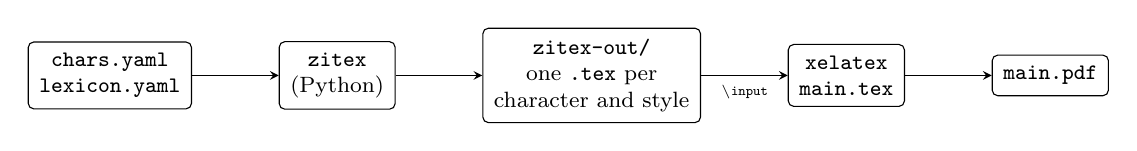
\begin{tikzpicture}[node distance=11mm, every node/.style={font=\footnotesize},
    box/.style={draw, rounded corners=2pt, align=center, inner sep=4pt}, >=stealth]
  \node[box] (yaml) {\texttt{chars.yaml}\\\texttt{lexicon.yaml}};
  \node[box, right=of yaml] (py) {\texttt{zitex}\\(Python)};
  \node[box, right=of py] (snip) {\texttt{zitex-out/}\\one \texttt{.tex} per\\character and style};
  \node[box, right=of snip] (xe) {\texttt{xelatex}\\\texttt{main.tex}};
  \node[box, right=of xe] (pdf) {\texttt{main.pdf}};
  \draw[->] (yaml) -- (py);
  \draw[->] (py) -- (snip);
  \draw[->] (snip) -- node[below, font=\tiny]{\cmd{input}} (xe);
  \draw[->] (xe) -- (pdf);
\end{tikzpicture}
\end{center}

\begin{center}
\small
\begin{tabular}{@{}p{0.27\linewidth}p{0.42\linewidth}p{0.22\linewidth}@{}}
\toprule
Half & Does & Written in \\
\midrule
\texttt{zitex} command & parse a shape, check positions, choose a layout, compute coordinates, look up pinyin and glosses, resolve fonts, write \LaTeX{} & Python \\
\texttt{zitex.sty} & load the packages the snippets need, define the \cmd{zi} commands, find and \cmd{input} the right snippet & \LaTeX{}, about 60 lines \\
\bottomrule
\end{tabular}
\end{center}

The document never contains a decomposition. It contains \cmd{zimath}\texttt{\{字\}}, and \LaTeX{} finds the snippet that Python wrote for that character.

\subsection{Why not do it all in \LaTeX{} macros?}
\begin{itemize}
  \item \textbf{Parsing is awkward in \TeX.} A shape string is a nested prefix expression with fixed arities, named groups and several kinds of operator. In Python it is a short recursive function.
  \item \textbf{Layout needs arithmetic and tables.} The matrix is laid out recursively, and the flat patterns need a small solver.
  \item \textbf{Data does not belong in a document.} Decompositions, roles, glosses and fonts live in YAML files that people review, test and check (\texttt{zitex check}). \LaTeX{} never sees them.
\end{itemize}
So the \LaTeX{} side is kept simple on purpose: it knows only file names.

\subsection{What \texttt{zitex.sty} does}
\begin{enumerate}
  \item \textbf{Loads what the snippets need:} \texttt{fontspec}, \texttt{xeCJK}, \texttt{amsmath}, \texttt{graphicx}, \texttt{tikz} and \texttt{xkeyval}. This is why \texttt{zitex} needs Xe\LaTeX.
  \item \textbf{Sets the Chinese font} (\cmd{setCJKmainfont}) and declares the operators \texttt{∴ ∵ ∷} part of the \texttt{CJK} class with \cmd{xeCJKDeclareCharClass}, so that \texttt{xeCJK} typesets them in the CJK font. Without it they print as nothing.
  \item \textbf{Defines the commands} \cmd{zi}\texttt{[style=, lang=, reading=]}, the four shortcuts, and \cmd{zitexsetlang}, \cmd{zitexsetreading}, \cmd{zitexsetpath}.
  \item \textbf{Includes the snippet, or says it is missing:} if the file exists, \cmd{input} pastes it in. If not, \LaTeX{} prints a warning and shows a red mark, so a missing snippet never stops a long build.
  \item \textbf{Avoids one trap:} an empty macro made with \cmd{newcommand} is not \cmd{ifx}-equal to one made with \cmd{def} (the first is \cmd{long}), so the package uses \cmd{def} for the reading.
\end{enumerate}

\subsection{The file name is the contract}
Python writes the snippets and the package reads them, and the only interface between them is the file name:

\begin{syntax}
\begin{verbatim}
zitex-out/u<hex>-<style>[-<lang>][@<reading>].tex     (u<hex>: the code point in hex)
\zimath[lang=fr, reading=dictionary]{虹}   ->   zitex-out/u8679-math-fr@dictionary.tex
\end{verbatim}
\end{syntax}

The language is part of the name only for the styles that print glosses (\texttt{math}, \texttt{formula}), and \texttt{@reading} only when a reading was asked for. The rule exists twice, in Python (\texttt{snippet\_name}) and in the package (\cmd{zitex@name}), and a test fails if they differ.

\subsection{What a snippet is}
Python writes one self-contained file per character and style.

\begin{center}
\small
\begin{tabular}{@{}lp{0.72\linewidth}@{}}
\toprule
Style & Snippet \\
\midrule
\texttt{math}    & plain \LaTeX{} math (\cmd{overset} for pinyin, \cmd{underbrace} for the gloss, \cmd{xrightarrow} for the reason), which MathJax and KaTeX also accept \\
\texttt{formula} & one line of text: parts, an arrow, the character, its pinyin and gloss \\
\texttt{matrix}  & TikZ, with rectangle coordinates that Python computed, and a fill colour from the role of each part \\
\texttt{tree}    & TikZ, one node per component at computed coordinates; Python does the layout, not a TikZ tree library \\
\bottomrule
\end{tabular}
\end{center}
Colours are defined inside every snippet, so it works when \cmd{input} into any document. A snippet that needs a special font carries its own helper commands, declared with \cmd{providecommand} so that they never clash with the package.

\subsection{Fonts and glyphs that are not in the font}
A component may be missing from the main font: a rare character, or a component with no Unicode code point. Python checks each component against the font files, and writes one of four forms:

\begin{center}
\small
\begin{tabular}{@{}p{0.38\linewidth}p{0.55\linewidth}@{}}
\toprule
Situation & What Python writes \\
\midrule
the font has the glyph      & the character itself \\
a fallback font has it      & a group that switches the CJK font for that one character \\
it is drawn as an image     & the image, included at text height \\
nothing can draw it         & a boxed label such as \texttt{U+20009}, and a warning in the build output \\
\bottomrule
\end{tabular}
\end{center}

\subsection{How the pieces find each other}
\begin{enumerate}
  \item \texttt{zitex extract} (or \texttt{zitex render --scan main.tex}) reads the paper as text, notes the character, style, language and reading of each \cmd{zi} command, and renders exactly those snippets into \texttt{zitex-out/}. It follows \cmd{zitexsetlang} and \cmd{zitexsetreading} in order, as the package does, and it skips comments and verbatim listings.
  \item \texttt{xelatex main.tex} loads \texttt{zitex.sty}. In a folder made by \texttt{zitex setup}, the package sits next to \texttt{main.tex}, so nothing is installed anywhere else. \texttt{zitex install-sty} installs it for all documents.
  \item At each \cmd{zi} command, the package builds the file name and \cmd{input}s \texttt{zitex-out/<name>.tex}. The folder is relative to where \texttt{xelatex} runs, and \cmd{zitexsetpath} changes it.
\end{enumerate}

\subsection{Readings}
Which part of a character carries the meaning and which the sound is an interpretation, and a character can store several. The reading chosen only changes the colouring and the arrow label, and never the structure. It reaches Python through the file name, so the \LaTeX{} side needs no new logic.

\end{document}
